\section{Method}
\label{sec:method}

In this section we present the theory applied in this work. 
we present our theoretical framework for expanding actor-critic RL algorithms with Ensemble methods, which we call the Generalized Critic. We start by giving a visual representation with an illustrative example to establish the intuition behind this practical view. We then move on to a more technical definition of each element.

\subsection{Generalized Critic}

For our practical case, we consider the case of an infinite horizon MDP. The set of actions $\mathcal{A}$ and the set of states $\mathcal{S}$ are continuous. $\pi_\theta$, the estimated policy with parameters $\theta$, is a gaussian probability distribution.

Let us consider the following scenario of a policy update: 
at epoch $k+1$, the current policy $\pi_{\theta_k}$ is used to sample training data from the environment through a cycle of actions ($a_t$) and feedback (the next state $s_{t+1}$, and the reward $r_t$). This execution scenario starting from the initial state $s_0$ up to the final state is called an \emph{episode}. The set of all states, actions and rewards the agent has experienced in an episode is called a \emph{trajectory}. 

The training sample of each epoch is a set $\mathcal{D}_k$ containig a given number of trajectories; in implementations, this corresponds to the minibatch for each update. The critic will update the estimator $\hat{V}(s_t)$ based on the new data, after which the advantage function is estimated. Following that, the policy update is performed, guided by the advantage function. There are several methods to optimize the policy gradient, so the specifics of this update will depend on the used algorithm.

As shown in figure \ref{fig:model}, we bring two additions to the standard scenario: the Generalized Critic, an Ensemble-based value function approximation, and the Aggregation Function $\mathcal{F}$ which combines the multiple estimates into a single output.


%We Actor-Critic

%Actor  policy gradient method

%Critic value function estimation

%We introduce diversity through various ways

%We average the 

\subsection{Variations}

Ensemble Learning is the foundation of the Generalized Critic method. The ability to introduce diversity in the models is therefore critical if we hope the final ensemble will average to an output that outperforms that of a single model. 

The potential of our method can be expanded through its combination with additional existent techniques, which can each add a unique element that contributes to strengthening the Ensemble. A very desirable outcome would be to help the model converge toward a good solution without generating additional data. Additionally, it may help control part of the stochasticity that is inherent to policy gradient methods and reduce the variance between each run.

Below are techniques to create potential variants of our method:

\begin{description}
\item[Estimation methods for the value and advantage functions]

%we can introduce diversity while estimating the advantage function.

%we can uuse gae

%we can use idk what ill check

%also if we use gae we can change parameters
%neat huh

%method
%gamma and lambda

\item[Random initialization and bootstrap at training]

The neural network estimator is initialized using random values, so as to diminish the noise produced by the initial values of a single model. When we train the network, we use a bootstrap\cite{efron1982jackknife} technique whereby at each update of the ensemble of value networks, we sample for each network different values from our collected trajectories following a Bernoulli distribution.

\item[Aggregation Function] The way that the different estimates are combined results in different possible values for the final output, some of which may be more advantageous than others depending on the context.


\item[Hyperparameters and optimizations]

\end{description}


The full process is detailed in the following algorithm:
\\
\label{sec:meth}
\begin{algorithm}[H]
\DontPrintSemicolon
  
  \KwInput{Initial actor network parameters $\theta_0$, initial critic parameter list $\phi^0_0, \dots, \phi^n_0$}
  %\KwOutput{Your output}
  %\KwData{Testing set $x$}

  \For{$i \leftarrow 1$ \KwTo total number of updates}{     
\While{buffer is not full}{     
  \tcc{collect set of trajectories $\mathcal{D}_k$}
         Run $\pi_{\theta_{old}}$ to generate an action
         
         Store the current state, action, and reward in buffer
         
         \If{episode ends}
         	{break}
   }
   
\If{episode was interrupted (buffer is full before episode end)}{
	\tcc{bootstrap remaining values}
	Run critic ensemble on last observation
	
	Combine estimates using the aggregation function
	
   }

  \For{$i \leftarrow 1$ \KwTo number of critics}{
   Estimate the advantage functions $\hat{A_i}$ using any (or several) estimation methods}

   Compute the PPO-CLIP policy loss as: %formula
   \[
   \theta_{k+1} = \argmax_{\theta} \frac{1}{\mathcal{D}_kT}\sum_{r \in |\mathcal{D}_k|}\sum^T_{t=0}\min \left(\frac{\pi_\theta(a_t|s_t)}{\pi_{\theta_k}(a_t|s_t)}A^{\pi_{\theta_k}}(s_t,a_t), g(\epsilon, A^{\pi_{\theta_k}}(s_t,a_t))\right)
   %{}{}
   \]
   
   Update the policy network

  \For{$i \leftarrow 1$ \KwTo number of critics}
    {
    	Update the value network $V_{\phi^1}$ by regression on mean-squared error:
    \[
    \Phi_{k+1} = \argmin_{\Phi} \frac{1}{|\mathcal{D}_k|T}\sum_{r\in \mathcal{D}_k}\sum^T_{t=0}\left(V_\Phi(s_t)-\hat{R_t}\right)^2
    \]
    }
}    
\caption{PPO-CLIP with Generalized Critic Policy Optimization}

\end{algorithm}

\begin{figure}[!htb]
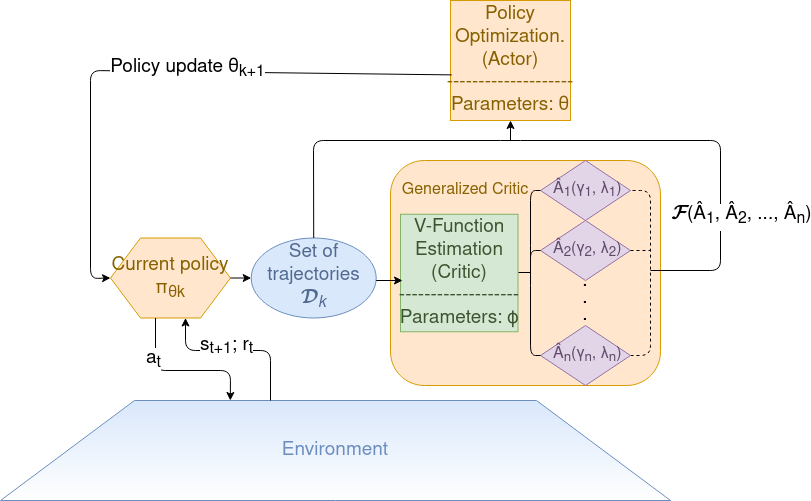
\includegraphics[width=\linewidth]{images/model}
\caption{Policy update scenario with a generalized critic.}
\label{fig:model}
\end{figure}


